% Chapter 1
\chapter{Underlay Network}
\section{OpenvSwitch architecture}

When a packet first arrives to the switch it is sent straight to the controller to take the decisions of what to do with the packet if dropping the packet or setting a new flow entry for forwarding future similar packets.\\

The OpenVSwitch design is divided in two parts the kernel module and the userspace.
The kernel module follows the instructions and allocate some cached results.\\

In the userspace the ovs-switch matches the packets and openflow tables and then it sends this information to the controller to be stored in the ovsdb-server,  \autoref{fig:ovs} shows the process for the first packets and the different path for consecutive packets, with an example of sending them to Virtual machines.\\


\begin{figure}[bth]
{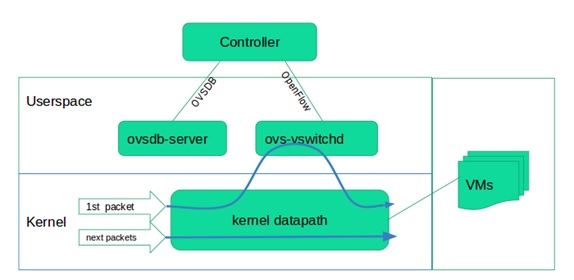
\includegraphics[width=1.2\linewidth]{gfx/ovs}}\caption[OpenvSwitch Architecture]{OpenvSwitch Architecture}
{\label{fig:ovs}
\end{figure}

\section{Containers} 


Containers are processes that are isolated from the rest of the machine, it can encapsulate any application dependencies, multiple applications can coexist in the same environment, it also speedup the application development by building the application only once and being able to run in every kind of environment, all containers share the same kernel unlike virtual machines, containers need only the necessary programs to run any kind of application or service without the need of an Operating system running on top of it, therefore they are more lightweigth than virtual machines.\\

Main characteristics applied to the model\\

Docker containers add a new layer of virtualization to the environment one physical device can have many virtual machines and on each virtual machine there can be many containers; for the containers to communicate with Virtual machines and within other containers, the inter-connection is not as straightforward as traditional topologies.\\

Since docker containers can access the kernel, docker provide a feature that will control the restrictions of the view of the system, namespaces are the ones that verify whether a user is allowed to access a specific file, process, etc.\\

To get an insight of the network infrastructure of docker containers, I used the the paper of Virtualization-A highlight on performance \cite{3} written by my previous tutor Guillaume Urvoy-Keller, and various docker tutorials\cite{4}. I used all the information and summarized them in the next section for the development of this project.\\

\section{Practical experimentation and issues}

This project was developed in a PC with 8,00GB of RAM and a quad-core processor, I installed Ubuntu on a dual boot and on the top of the Ubuntu Operating system I installed the Docker infrastructure.\\

First it is important to know that docker containers create by default a docker0 network that at the moment a container start running it creates a veth peer link to the docker network and create a new network namespace in the container. To  eliminate this docker network while running a new container we can specify that we don’t want any network description to be attached to our running container with the flag –net=’none’   or we can  bring docker 0 down.\\

This will help in the future to avoid problems at the moment of appending to the underlying network and for migration of containers.\\
\begin{itemize}
\item Creation of a New container:\\
\texttt{docker run --name=controller --net='none' -ti ubuntu /bin/bash}\\
\item Two containers linked with the use of namespace:\\
This information is important since in the installation of the services of Open Stack we can see also the same way of configuring different nodes for stating the service that is going to be the controller.\\
\texttt{docker run -ti --name compute --link controller:controller ubuntu /bin/bash}\\
This command links a container that was previously created (controller) with a new container created called compute, but it is only a one way connection, so for the compute node I created  the \texttt{/etc/hosts} file as well.
\item Two containers with OpenvSwitch:\\
\texttt{ovs-vsctl add-br s1}\\
\texttt{ifconfig br1 192.168.0.1 netmask 255.255.255.0}

\end{itemize}

Since docker containers have assigned each a unique namespace we have to create also the network namespace, for doing this we need to check the process id of the container that we are planning to join to my network and store its value in the file \texttt{/var/run/netns}\\

To save the process id of the controller:\\
\texttt{docker inspect -f '{{.State.Pid}}' <process id of c1>}\\
After this we get the process id and we create a namespace entry in \texttt{/var/run/netns} to specify the connection.\\

\texttt{pid=} #here we have to write the new process id\\
\texttt{mkdir -p /var/run/netns}\\
\texttt{ln -s /proc/$pid/ns/net /var/run/netns/$pid}\\

Note: to check the process id: \texttt{docker ps}\\
 
Next it was created a peer of interfaces c1-eth0 corresponding to the network namespace of the container c1 and s1-eth1 corresponding to the OpenvSwitch s1 that was previously created; next it was assigned an ip and a default route \autoref{fig:dockerconnected}, shows this architecture.\\

\begin{figure}[bth]
{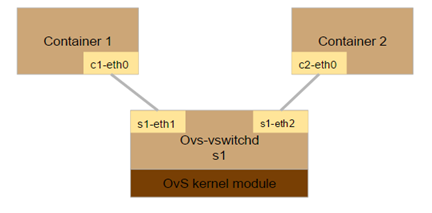
\includegraphics[width=0.7\linewidth]{gfx/dockerconnected}}\caption[OpenvSwitch connected with 2 docker containers]{OpenvSwitch connected with 2 docker containers}
{\label{fig:dockerconnected}
\end{figure}


For the creation of the peer interfaces c1-eth0 and s1-eth1, and for binding s1-eth1 to the bridge s1 I did the next:\\

\texttt{ip link add c1-eth0 type veth peer name s1-eth1}\\
\texttt{ovs-vsctl add-port s1 s1-eth1}\\
\texttt{ip link set s1-eth1 up}\\

Next to bind c1-eth0 to the container network namespace assigning an ip\\

\begin{lstlisting}[language=bash,frame=tb,caption={Network namespaces creation}]
ip link set c1-eth0 netns $pid
ip netns exec $pid ip link set c1-eth0 address 12:34:56:78:9a:bc
ip netns exec $pid ip link set c1-eth0 up
ip netns exec $pid ip addr add 192.168.0.0/24 dev c1-eth0
ip netns exec $pid ip route add default via 192.168.0.1
\end{lstlisting}\\

All this experimentations provide different ways for containers to be inter-connected, attaching containers together, using linux bridges or docker containers, but since in the next part of the work I will be using Multi-host configuration and I will need to configure OpenStack Self Services, I tried it with OpenVSwitch and Linux Bridge to choose the best in performance.\\

To choose the right approach I have tested different situations and architectures.
I used docker containers since they are more lightweight than hypervisors they can run up to 10.000 of containers in one host, containers use cgroups and namespaces.\\

\section{Analysis}
\subsection{Linux bridge vs OpenvSwitch}\\

When we run a new container or when several containers run they by default a create a linux bridge for connectivity, the problem with linux bridges is that it has a limit in scalability, since Docker containers and Openstack Virtual machines are in two different level of virutalization the best aproach is to use OpenvSwitch.\\

\subsubsection{Benchmarking}

Cpu Benchmarking:\\

First I had use Docker containers and Vagrant virtual machines using sysbench  with  1000 of computations for computing prime numbers with 2 CPUs available reaching a result that the time average to perform the computation on a docker container was almost half quick as the time on Vagrant virtual machines.\\

Network Benchmarking \\

For the network benchmarking I run two nodes one as a client \texttt{iperf -c} and the other as a server \texttt{iperf -s} and transferring messages with the results shown in the next chart we can see that Docker with OVS is a faster approach.\\

Ipef is used to check the network bandwith and the quality of the link.\\

\autoref{fig:benchmark} presents the throughput of the iperf command by sending messages from 64MB with the -m option and so on decreasing the bandwith 

\begin{figure}[bth]
{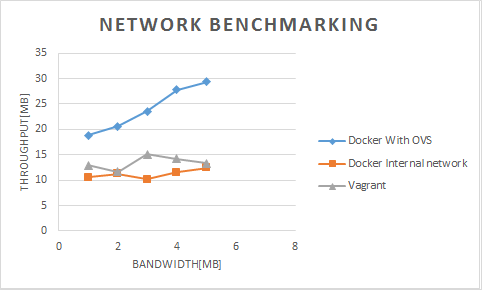
\includegraphics[width=1.2\linewidth]{gfx/benchmark}}\caption[Throughput: performance after iperf command]{Throughput: performance after iperf command}
{\label{fig:benchmark}
\end{figure}\\

The partial conclusion of this part of the project explains why I chose to use a Docker container with OpenvSwitch since as shown in the figure above this architecture has a more efficient support. 

\marginpar{Docker with ovs provide a better throughput specially for smaller bandwidth}

\subsection{Docker engine}

Docker uses a docker engine, which manages with the docker daemon the interaction between container and use of the resources of system, information of the containers such as process ID's, state of the containers, create,  stop, run, execute, remove a container, etc.\\ 

Docker solves the problem of dependencies of the binaries and libraries, \autoref{fig:dockerarchitecture} represents the architecture of docker containers and shows how docker is detached from the Guest Operating system and how the docker engine manages all the processes. Because of this any application that is created on docker is independent of the operating system in which docker is running.\\

\begin{figure}[bth]
{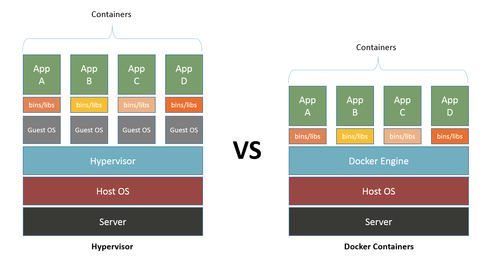
\includegraphics[width=1\linewidth]{gfx/dockerarchitecture}}\caption[Docker vs virtual machines architecture]{Docker vs virtual machines architecture \cite{14}}
\label{fig:dockerarchitecture}
\end{figure}\\


Docker daemon must reload every time a new docker system is added to the environment this information will be very useful for further steps in this project.\\

Docker containers simplifies the complexity of installation and development of flexible cloud models, having many options of cloud infrastructures, the most straightforward way to start a new cloud architecture is using repositories with the minimal architecture and then adding different options for specific business\\

\subsection{Docker with OpenStack}

Docker containers can run any kind of software they are configured to run, to know how to configure each container it is important to know the different functions that docker can offer, the docker engine provides fast to test and deploy applications.\\

To develop the configuration of this applications docker engine uses dockerfile. Dockerfile contains the configuration that the service needs, it has a mix of linux commands and docker commands for installation of packages.\\

For the configuration of the container to be saved, it is needed to commit the changes and save them, we can also save them in a repository, Docker has a SaaS service for sharing a repository called Dockerhub.\cite{4}\\

In this part of the project I pulled a container from the repository continues/openstack-controller, continues/openstack-network, continues/openstack-compute that has the basic configuration of OpenStack, and added the respective configuration provided by OpenStack self-services in the next section there is the explanation of the motive to choose OpenStack Self Services.\\

Example of dockerfile:\\
\begin{lstlisting}[language=yaml,frame=tb,caption={Dockerfile}]
FROM ubuntu:14.04
RUN apt-get update \
	&& apt-get -y install software-properties-common python-software-properties \
	&& add-apt-repository -y cloud-archive:mitaka \
	&& apt-get update \
	&& apt-get -y dist-upgrade \
	&& apt-get -y install python-mysqldb 
RUN apt-get -y install neutron-plugin-ml2 neutron-plugin-openvswitch-agent \
    neutron-l3-agent neutron-dhcp-agent
EXPOSE 9696
\end{lstlisting}\\

Note: To save the containers configuration\\
\texttt{Docker commit <process id> anabeldlw/openstack<service>:<version>}\\

After commiting the configuration of the container we need to tag and push them to the repository.\\

First we learn the image id with the docker images command, then we need to copy the id for the name of the image as shown in the next example:\\
\begin{lstlisting}[language=yaml,frame=tb,caption={Dockerfile}]
$docker images
REPOSITORY				       TAG	 IMAGE ID	   CREATED 	    SIZE
anabeldlw/openstack_controller	tag1 71c0daa71ae8 3 days ago 	718MB

$docker tag 71c0daa71ae8 anabeldlw/openstack_controller:tag1
$docker push anabeldlw/openstack_controller:tag1
\end{lstlisting}\\

\subsection{Network configuration on OpenStack}

In this section there will be an explanation of the Self-service networks and the provider networks and the reason for choosing the Self-service networks.\\

\section{Provider networks}

Provider networks are managed only by administrators, since they need the configuration of a physical network infrastructure. This networks only handle layer 2 connectivity for instances\\

\subection{Self-service networks}

The advantage of the self-service networks over the provider network is that with self-services it is possible to enable projects to manage networks totally virtual and without the need of  involving administrators.\\

The support of networks without overlapping IP addresses will be done by the use of the VXLAN and GRE protocols, in contrast to the provider networks that are using layer 2 segmentation.\cite{6} \\

IPv4 usually use private IP addresses according to RFC7348 \cite{7}  with NAT and floating IP \\

This network service use Layer 3 routers that reside in a network node in contrary to provider networks that rely in physical network. \\

After reviewing this descriptions for the network configuration of OpenStack I reached to the conclusion that for the network configuration of OpenStack to work in concordance with the one of docker containers, it needs to be the one fully virtualized, network self services.\\

The requirements for the Self-service network are the next:\\

\begin{itemize}
\item 2 network interfaces (management and provider)
\item sql service with  databases for OpenStack
\item keystone, glance, nova 
\item neutron and ML2 plugin
\end{itemize}

For the configuration of the VXLAN in the controller node, the VNI has to be chosen and as specified in the RFC7348 document \\

“The VNI is in an outer header that encapsulates the inner MAC frame originated by the VM”.\cite{7}  \\

This document explain how the VNI is used for the encapsulation of inner MAC addresses produced by virtual machine addresses so if there is an overlapping of physical and virtual machine addresses, the VNI will identify the inner virtual machine addresses.\\